% !TEX TS-program = pdflatex
% !TEX encoding = UTF-8 Unicode

\documentclass[a4paper, titlepage=false, parskip=full-, 10pt]{scrartcl}

\usepackage[utf8]{inputenc}
\usepackage[T1]{fontenc}
\usepackage[english, ngerman]{babel}
\usepackage{babelbib}
\usepackage{hyperref}
\usepackage{listings}
\usepackage{framed}
\usepackage{color}
\usepackage{graphicx}
\usepackage[normalem]{ulem}
\usepackage{cancel}
\usepackage{amsmath}
\usepackage{amssymb}
\usepackage{amsthm}
\usepackage{algorithm}
\usepackage{algorithmic}
\usepackage{geometry}
\usepackage{subfigure}
\geometry{a4paper, top=20mm, left=35mm, right=25mm, bottom=40mm}

\newcounter{tasknbr}
\setcounter{tasknbr}{1}
\newenvironment{task}[1]{{\bf Aufgabe \arabic {tasknbr}\stepcounter{tasknbr}} (#1):\begin{enumerate}}{\end{enumerate}}
\newcommand{\subtask}[1]{\item[#1)]}

% Listings -----------------------------------------------------------------------------
\definecolor{red}{rgb}{.8,.1,.2}
\definecolor{blue}{rgb}{.2,.3,.7}
\definecolor{lightyellow}{rgb}{1.,1.,.97}
\definecolor{gray}{rgb}{.7,.7,.7}
\definecolor{darkgreen}{rgb}{0,.5,.1}
\definecolor{darkyellow}{rgb}{1.,.7,.3}
\lstloadlanguages{C++,[Objective]C,Java}
\lstset{
escapeinside={§§}{§§},
basicstyle=\ttfamily\footnotesize\mdseries,
columns=fullflexible, % typewriter font look better with fullflex
keywordstyle=\bfseries\color{blue},
% identifierstyle=\bfseries,
commentstyle=\color{darkgreen},      
stringstyle=\color{red},
numbers=left,
numberstyle=\ttfamily\scriptsize\color{gray},
% stepnumber=5,
% numberfirstline=true,
breaklines=true,
% prebreak=\\,
showstringspaces=false,
tabsize=4,
captionpos=b,
% framexrightmargin=-.2\textwidth,
float=htb,
frame=tb,
frameshape={RYR}{y}{y}{RYR},
rulecolor=\color{black},
xleftmargin=15pt,
xrightmargin=4pt,
aboveskip=\bigskipamount,
belowskip=\bigskipamount,
backgroundcolor=\color{lightyellow},
extendedchars=true,
belowcaptionskip=15pt}

%% Enter current values here: %%
\newcommand{\lecture}{Algorithmische Geometrie SS15}
\newcommand{\tutor}{}
\newcommand{\assignmentnbr}{3}
\newcommand{\students}{Julius Auer, Alexa Schlegel}
%%-------------------------------------%%

\begin{document}  
\lstset{language=Java}
{\small \textsl{\lecture \hfill \tutor}}
\hrule
\begin{center}
\textbf{Übungsblatt \assignmentnbr}\\
[\bigskipamount]
{\small \students}
\end{center}
\hrule

\begin{task}{Graham-Scan}\item[]
\emph{Implementieren Sie den Graham-Scan. Benutzen Sie dabei aus Gründen besserer Laufzeit und zur Vermeidung von Rundungsfehlern möglichst nur die Grundrechenarten $+,-,\times, \div$. Eine Umrechnung in Polarkoordinaten, wie in der Vorlesung beschrieben, ist nicht nötig, um die Strahlen nach Steigung zu sortieren.}

Im Folgenden wird der implementierte Algorithmus mit Hilfe von Pseudocode beschreiben, dieser orientiert sich an der in \emph{Introduction to Algorithms}\footnote{Introduction to Algorithms, Second Edition, S. 949} vorgestellten Lösung. Der Stack $S$ wird verwendet, um mögliche Kandidaten der konvexen Hülle zu verwalten. Nach terminierung des Algorithmus enthält $S$ die Knoten der konvexen Hülle entgegen dem Urzeigersinn.

\begin{algorithm}
\caption{Graham-Scan(Q)}
\begin{algorithmic}[1]
\STATE sei $p_0 \in Q$ mit minimaler $y$-Koordinate:\\
bei gleicher $y$-Koordinate wird minimale $x$-Koordinate verwendet
\STATE sei ${p_1, p_2, \dots, p_n}$ die restlichen Punkte aus $Q$:\\
von $p_0$ aus gesehen in Polarkorrdinaten gegen den Urzeigersinn sortiert\\
bei gleichem Winkel, nur Punkt mit größtem Abstand von $p_0$ behalten\\
\STATE \textsc{Push}($p_0$, $S$)\\
\STATE \textsc{Push}($p_1$, $S$)\\
\STATE \textsc{Push}($p_2$, $S$)\\
\FOR{$i=3$ \TO $n$}
    \WHILE{Winkel (\textsc{Next-To-Top}($S$), \textsc{Top}($S$), $p_i$) ist keine Linkskurve}
    \STATE \textsc{Pop}($S$)
    \ENDWHILE
    \STATE \textsc{Push}($p_i$, $S$)
\ENDFOR
\RETURN{$S$}
\end{algorithmic}
\end{algorithm}

Die Methode \emph{grahamscan()} erhält als Eingabe eine Punktwolke und liefert ein Polygon zurück, welches der Konvexenhülle dieser Punktwolke entspricht.

Wir verwenden als Startpunkt des Algorithmus den Punkt der am weitestens Links liegt und die kleinsten $y$-Koordinte besitzt (\emph{getMinY()}). (In der Vorlesung wird ein beliebiebiger Punkt in der Mitte der Punktwolke ermittelt.)

Die Sortierung der Punkte erfolgt nach ihrer Steigung. Damit die Punkte gegen den Urzeigersinn sortiert sind werden sie vorher an der Funktion $f(x)=|x|$ gespiegelt und erst dann der Anstiegt berechnet (\emph{getRelevantPoints()}).

Um Links- und Rechskurven zu prüfen, wird die Determinante einer $2x2$-Matrix bestimmt, welche sich aus den zwei Vektoren der folgenden drei Punkte zusammensetzt. $t$ ist der letzte Punkt auf dem Stack, $ntt$ der vorletzte Punkt und $ca$ der Punkt der aktuelle betrachtet wird. Es wird getestet ob $\overline{t~cp}$ links oder rechts von $\overline{t~ntt}$ liegt.

\newpage

\lstinputlisting[language=Java, firstline=18, lastline=85]{../../AlGeo/src/algorithms/ConvexHull.java}

\lstinputlisting[language=Java, firstline=18, lastline=34]{../../AlGeo/src/geometry/Points.java}

\lstinputlisting[language=Java, firstline=36, lastline=66]{../../AlGeo/src/geometry/Points.java}

\newpage

Zur Veranschaulichung des Algorithmus gibt es einen Testklasse, wo die einzelnen Schritte visualisiert werden. Hier ein Beispiel mit 10 zufälligen Punkten:

\begin{figure}[h]
\begin{center}
\subfigure{
    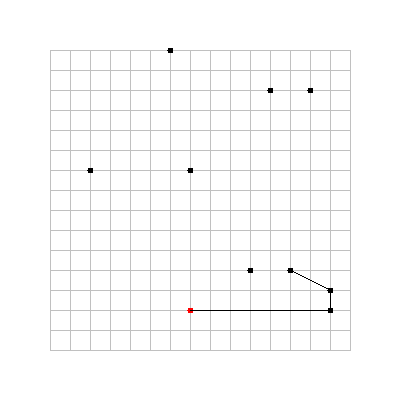
\includegraphics[width=5cm]{capture1}
}
\subfigure{
    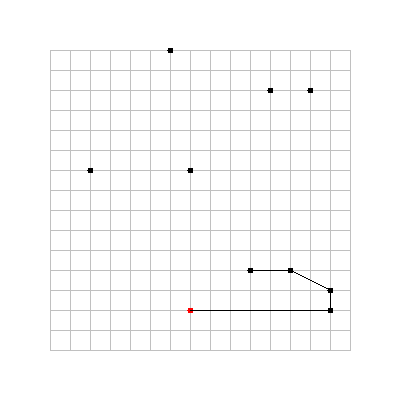
\includegraphics[width=5cm]{capture2}
}
\subfigure{
    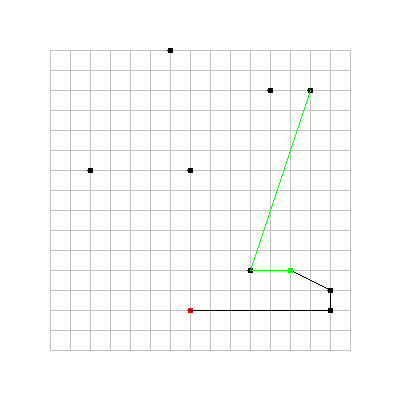
\includegraphics[width=5cm]{capture3}
}
\subfigure{
    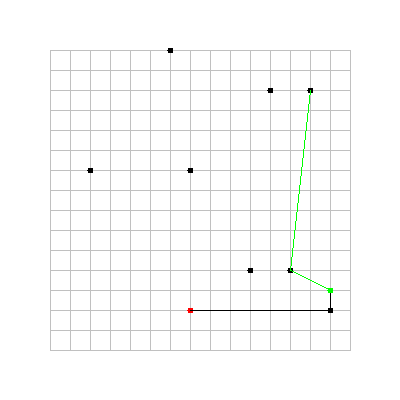
\includegraphics[width=5cm]{capture4}
}
\subfigure{
    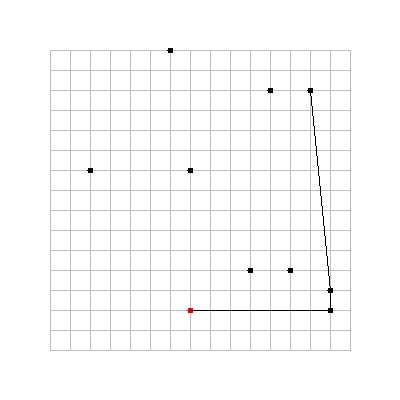
\includegraphics[width=5cm]{capture5}
}
\subfigure{
    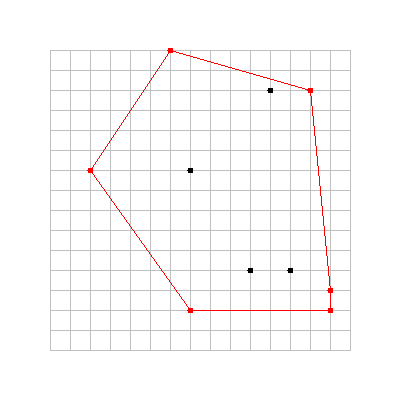
\includegraphics[width=5cm]{capture12}
}
\end{center}
\caption{Die ersten 5 Schritte und die resultierende Konvexehülle.}
\end{figure}

\end{task}

\begin{task}{inkrementelle Konstruktion der konvexen Hülle}\item[]
Die ersten drei Punkte $S=p_1,p_2,p_3$ werden zunächst nach X-Koordinate aufsteigend und dann nach Y-Koordinate absteigend sortiert. Die konvexe Hülle $CH(S)=S$ ist somit ein Polygonzug der im Uhrzeigersinn verläuft. Ferner wird das Center of Mass $com=((x_1+x_2+x_3)/3,(y_1+y_2+y_3)/3)$ bestimmt. Außerdem wird als Datenstruktur ein binärer Suchbaum $T$ angelegt, der $search(p)$, $insert(p)$ und $delete(p)$ in $O(\log n)$ garantiert (z.B. ein AVL-Baum) - in diesen werden $p_1,p_2,p_3$ eingefügt, wobei die totale Ordnung gegeben ist durch
$$p_i<p_j\text{ g.d.w. }\frac{y_i-y_{com}}{x_i-x_{com}}<\frac{y_j-y_{com}}{x_j-x_{com}}$$
wenn also die Steigung zwischen $com$ und $p_i$ kleiner ist, als die von $com$ und $p_j$. Diese Ordnung gilt auch für zukünftige Operationen auf dem Baum. $search(p)$ soll hierbei den Punkt aus $CH(S)$ liefern, der die nächst kleinere Steigung im Vergleich zu $p$ hat. Diese Initialisierung benötigt offensichtlich nur $O(1)$ Zeit.

Für jeden weiteren Punkt $p_n$ um den die konvexe Hülle $S=p_1,...,p_{n-1}$ erweitert werden soll wird nun $CH(S,p_n,T)$ aufgerufen, wobei $left(p,\overrightarrow q)$ die Funktion sei, die prüft ob $p$ auf der linken Seite des Vektors $\overrightarrow q$ liegt und $S.insert(p_i,j)$ den Punkt $p_i$ hinter dem Punkt $p_j$ zum Polygonzug $S$ der konvexen Hülle hinzufügt:
\begin{algorithm}
\caption{$CH(S,p_n,T)$}
\begin{algorithmic}[1]
\STATE$p_i=T.search(p_n)$\\
\IF{$left(p_n,\overrightarrow{p_ip_{i+1}})$}
\RETURN
\ENDIF
\STATE$T.insert(p_n)$\\
\STATE$S.insert(p_n,i)$\\
\STATE$j=i$\\
\WHILE{$left(p_n,\overrightarrow{p_{j-1}p_j})$}
\STATE$T.remove(p_j)$\\
\STATE$S.remove(p_j)$\\
\STATE$j-=1$\\
\ENDWHILE
\WHILE{$left(p_n,\overrightarrow{p_ip_{i+1}})$}
\STATE$T.remove(p_i)$\\
\STATE$S.remove(p_i)$\\
\STATE$i+=1$\\
\ENDWHILE
\end{algorithmic}
\end{algorithm}
\end{task}

Speicherplatz:\\
$O(n)$ für einen AVL-Baum.

Laufzeit:\\
Es bietet sich hier an, den Polygonzug in einer verketteten Liste zu speichern. Die Elemente der Liste werden stets über den Baum adressiert - was effizient ist - während in konstanter Zeit Zeiger umgelegt werden können. Für das Einfügen von $n$ Punkten muss $n\times$ \emph{CH(...)} ausgeführt werden. Dessen Zeitaufwand ergibt sich zu:
\begin{itemize}
\item $O(\log n)$ für das Suchen im Baum (1)
\item $O(1)$ für Listenoperationen (2-4, 6)
\item $O(\log n)$ für das Einfügen in den Baum (5)
\item $O(f(n))\cdot O(\log n)$ wobei die Größe von $f(n)$ im Folgenden zu untersuchen ist (8-17)
\end{itemize}

Anstatt über planare Graphen zu argumentieren ist hier vlt. eine sehr einfache Anwendung der Buchhalter-Methode möglich!?:

Jeder Punkt wird nur höchstens einmal zu der konvexen Hülle hinzugefügt und beim Hinzufügen mit einem Guthaben von '1' ausgestattet. Wird ein Punkt gar nicht zur konvexen Hülle hinzugefügt verbleibt er mit einem Guthaben von '0'. Beim Hinzufügen eines Punktes $p_i$ werden in den beiden Schleifen einmal der linke und einmal der rechte Nachbar inspiziert, was beim Hinzufügen von $n$ Punkten $O(n)$ Zeit benötigt. Nur wenn $p_{i-1}$ oder $p_{i+1}$ entfernt werden müssen, besteht die Notwendigkeit einen weiteren Punkt zu untersuchen. Für diesen zusätzlichen Schritt wird nun das Guthaben von $p_{i-1}$ bzw. $p_{i+1}$ aufgebraucht. $p_{i-1}$ bzw. $p_{i+1}$ werden in diesem Fall allerdings entfernt und verbleiben so mit einem Guthaben von '0'.\\
D.h.: neben konstant 2 Vergleichen pro Aufruf des Algorithmus wird jede Kante des Polygons bei der Suche nach zu Entfernenden Kanten höchstens 1 mal passiert (nach dem ersten Mal fliegt die Kante raus). Bei $n$-maligem Aufruf fallen somit nur Kosten von $O(n)$ an.

Die Gesamtlaufzeit ergibt sich somit zu $O(n\cdot\log n)$.

\begin{task}{untere Schranke}\item[]
Angenommen die konvexe Hülle der Punkte $S=\{(a_1,a_1^2),...,(a_n,a_n^2)\}$ ließe sich in weniger als $\Omega (n\cdot\log n)$ bestimmen. Die konvexe Hülle hat hier stets die Form $CH(S)=p_1,..,p_n$ mit $x_i\ge x_{i+1}$ und $y_i\ge y_{i+1}$ (vgl. auch Abb. 2).
\begin{figure}[htpb]
\begin{center}
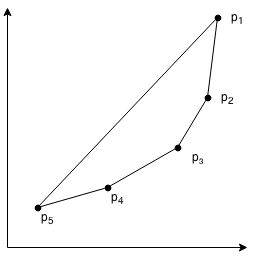
\includegraphics[width=5cm]{sketch1}
\end{center}
\caption{Konvexe Hülle (keine lineare Skala!)}
\end{figure}

Beweis (Induktion):\\
I.A.: Der Polygonzug $p_1,p_2,p_3$ aus 3 Punkten beschreibt offensichtlich immer eine konvexe Hülle.

I.V.: Der Polygonzug $p_1,...,p_n$ mit $x_i\ge x_{i+1}$ beschreibt die konvexe Hülle von $\{p_1,...,p_n\}$

$n\rightarrow n+1:$ Alle Punkte $p_1,...,p_n$ liegen rechts der Geraden $\overrightarrow{p_{n+1}p_1}$, da stets
\begin{align*}
&\frac{y_1-y_{n+1}}{x_1-x_{n+1}}>\frac{y_1-y_n}{x_1-x_n}\\
=&\frac{x_1^2-x_{n+1}^2}{x_1-x_{n+1}}>\frac{x_1^2-x_n^2}{x_1-x_n}
\end{align*}
(aufgrund der Tatsache, dass nach Voraussetzung $x_n\ge x_{n+1}$) und nach I.V. alle $p_i$ mit $i<n$ schon vorher rechts der Geraden $\overrightarrow{p_np_1}$ lagen. $p_n$ (und somit auch alle $p_i$ mit $i<n$) kann jedoch auf keinen Fall aus der konvexen Hülle ''gestrichen'' werden, da (nach derselben Rechnung) die Steigung von $\overrightarrow{p_np_{n-1}}$ steiler sein muss, als die von $\overrightarrow{p_{n+1}p_n}$. Damit muss die konvexe Hülle $CH(p1,...,p_{n+1})=p1,...,p_{n+1}$ sein.

Somit könnte man den Polygonzug in linearer Zeit ablaufen um die sortierte Folge $a_n,..,a_1$ zu erhalten (da stets $x_i\ge x_{i+1}$). Das Sortieren der Folge hätte somit nur soviel Zeit benötigt wie die Konstruktion der konvexen Hülle zzgl. $O(n)$ für das Berechnen der Quadrate und noch einmal $O(n)$ für das Ablaufen des Polygonzugs. Dies ist nach Annahme jedoch nicht möglich: die Konstruktion der konvexen Hülle muss folglich $\Omega (n\cdot\log n)$ Zeit benötigen.
\end{task}
\end{document}